\documentclass{standalone}
\usepackage{tikz}
\usetikzlibrary{patterns, positioning}
\usepackage[sfdefault]{ClearSans} %% option 'sfdefault' activates Clear Sans as the default text font
\usepackage[T1]{fontenc}

\begin{document}
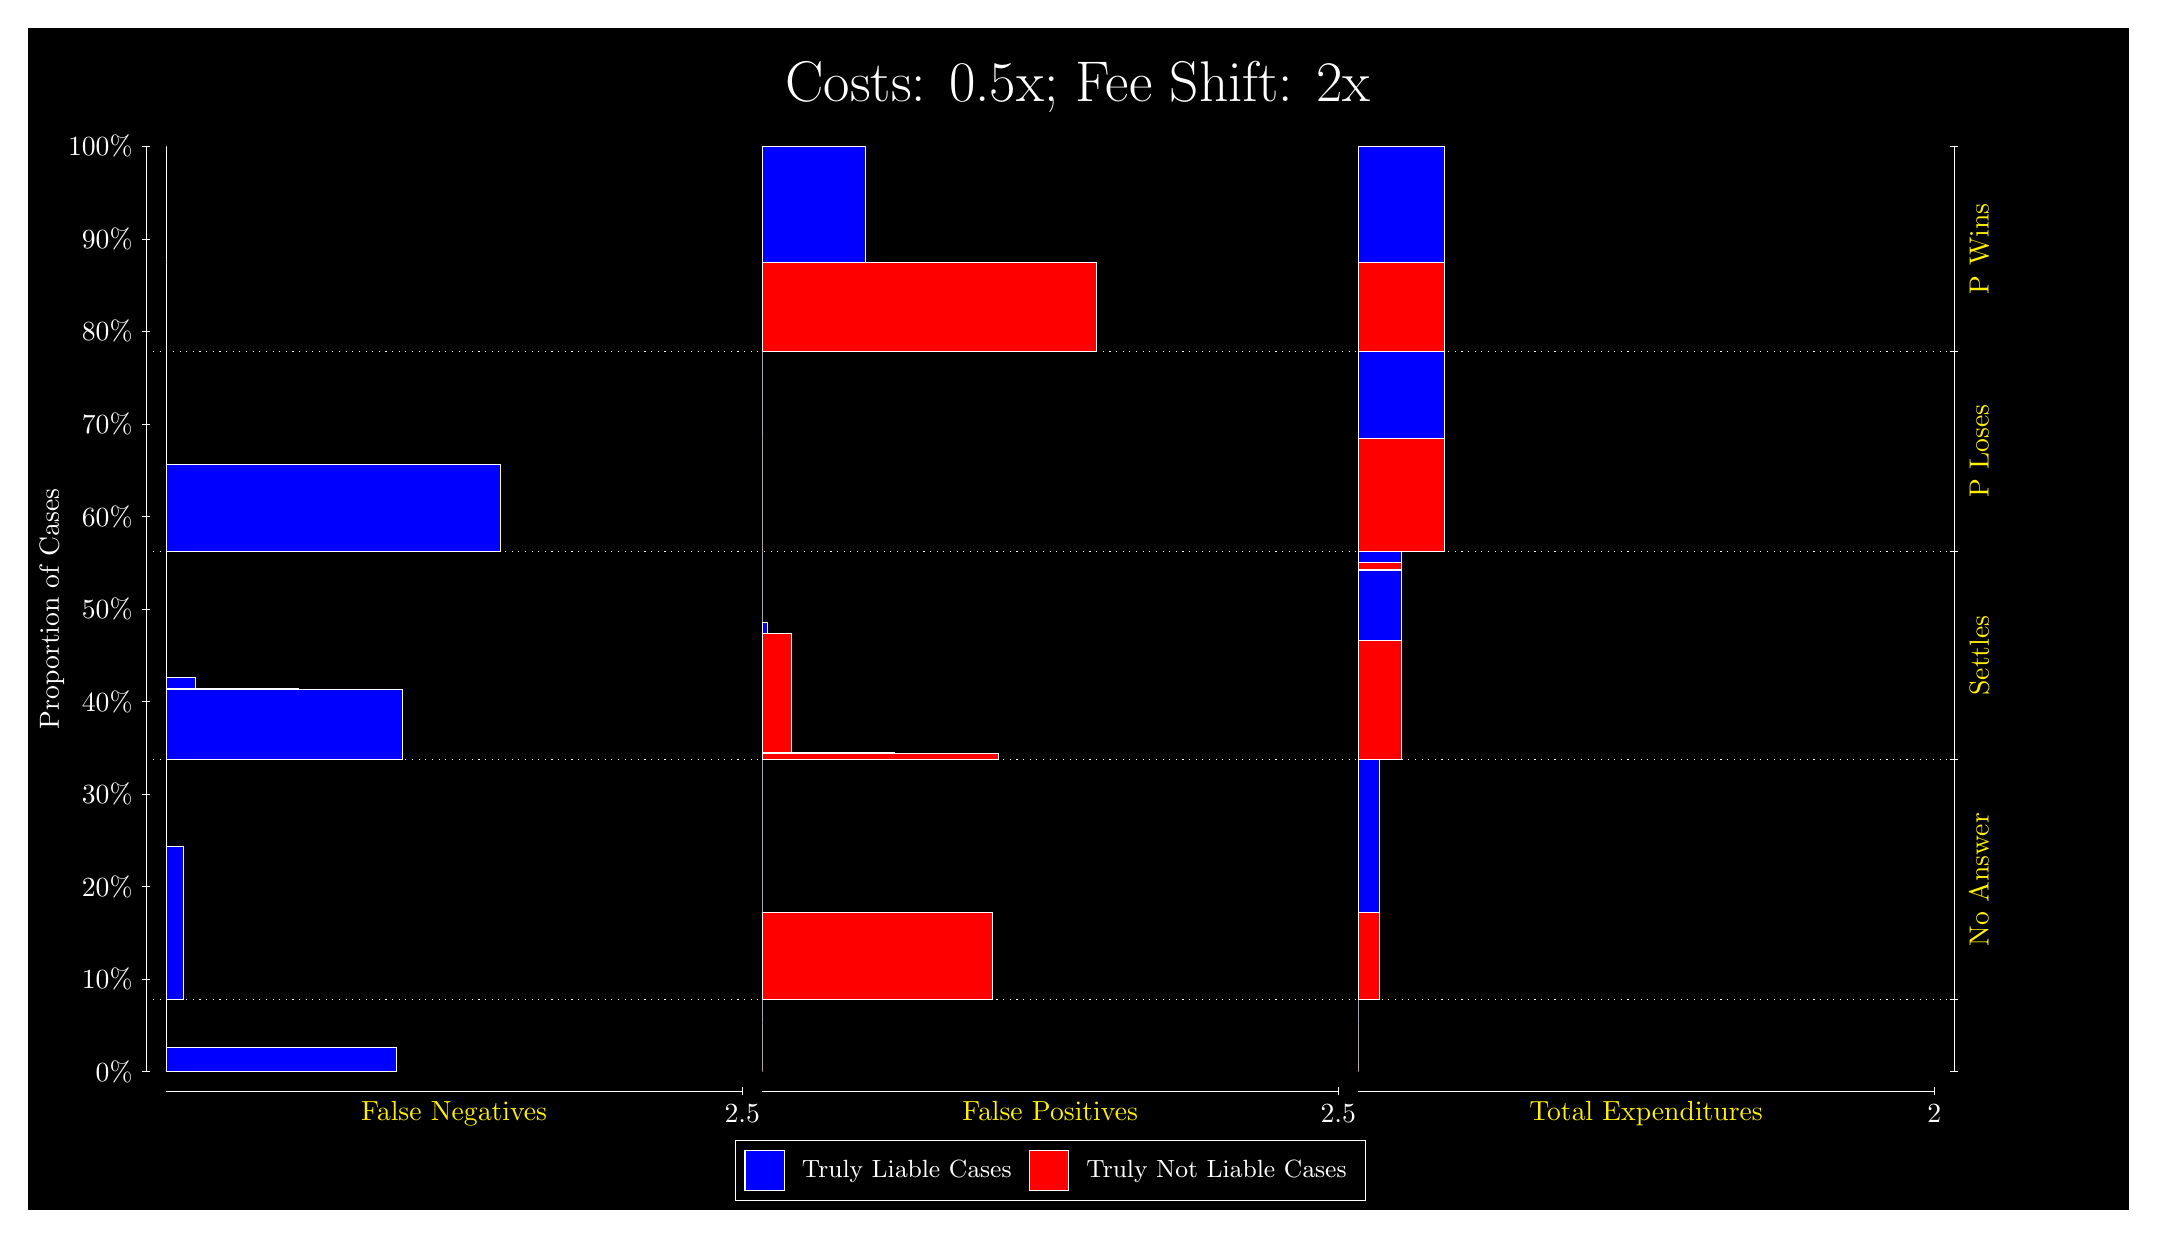
\begin{tikzpicture}
\draw[fill=black] (0,0) rectangle (26.667,15);
\draw[text=white] (0,13.5) rectangle (26.667,15) node[midway] {\huge Costs: 0.5x; Fee Shift: 2x};
\draw[white, very thin] (1.5,1.75) -- (1.5,13.5);
\node[rotate=90, text=white, anchor=center] at (0.3, 7.625) {Proportion of Cases};
\draw[white, very thin] (1.45,1.75) -- (1.55,1.75);
\node[text=white, anchor=east] at (1.45, 1.75) {0\%};
\draw[white, very thin] (1.45,2.925) -- (1.55,2.925);
\node[text=white, anchor=east] at (1.45, 2.925) {10\%};
\draw[white, very thin] (1.45,4.1) -- (1.55,4.1);
\node[text=white, anchor=east] at (1.45, 4.1) {20\%};
\draw[white, very thin] (1.45,5.275) -- (1.55,5.275);
\node[text=white, anchor=east] at (1.45, 5.275) {30\%};
\draw[white, very thin] (1.45,6.45) -- (1.55,6.45);
\node[text=white, anchor=east] at (1.45, 6.45) {40\%};
\draw[white, very thin] (1.45,7.625) -- (1.55,7.625);
\node[text=white, anchor=east] at (1.45, 7.625) {50\%};
\draw[white, very thin] (1.45,8.8) -- (1.55,8.8);
\node[text=white, anchor=east] at (1.45, 8.8) {60\%};
\draw[white, very thin] (1.45,9.975) -- (1.55,9.975);
\node[text=white, anchor=east] at (1.45, 9.975) {70\%};
\draw[white, very thin] (1.45,11.15) -- (1.55,11.15);
\node[text=white, anchor=east] at (1.45, 11.15) {80\%};
\draw[white, very thin] (1.45,12.325) -- (1.55,12.325);
\node[text=white, anchor=east] at (1.45, 12.325) {90\%};
\draw[white, very thin] (1.45,13.5) -- (1.55,13.5);
\node[text=white, anchor=east] at (1.45, 13.5) {100\%};

\draw[white, very thin] (24.457,1.75) -- (24.457,13.5);
\draw[white, very thin] (24.407,1.75) -- (24.507,1.75);
\node[anchor=west] at (24.407, 1.75) {};
\draw[white, very thin] (24.407,2.6669) -- (24.507,2.6669);
\node[anchor=west] at (24.407, 2.6669) {};
\draw[white, very thin] (24.407,5.711) -- (24.507,5.711);
\node[anchor=west] at (24.407, 5.711) {};
\draw[white, very thin] (24.407,8.3563) -- (24.507,8.3563);
\node[anchor=west] at (24.407, 8.3563) {};
\draw[white, very thin] (24.407,10.897) -- (24.507,10.897);
\node[anchor=west] at (24.407, 10.897) {};
\draw[white, very thin] (24.407,13.5) -- (24.507,13.5);
\node[anchor=west] at (24.407, 13.5) {};

\draw[white, very thin, fill=blue] (1.75,1.75) rectangle (4.6775,2.0594);
\draw[white, very thin, fill=red] (1.75,2.0594) rectangle (1.75,2.6669);
\draw[white, very thin, fill=blue] (1.75,2.6669) rectangle (1.9696,4.6096);
\draw[white, very thin, fill=red] (1.75,4.6096) rectangle (1.75,5.711);
\draw[white, very thin, fill=blue] (1.75,5.711) rectangle (4.7507,6.6047);
\draw[white, very thin, fill=blue] (1.75,6.6047) rectangle (3.4333,6.6112);
\draw[white, very thin, fill=blue] (1.75,6.6112) rectangle (2.1159,6.7508);
\draw[white, very thin, fill=red] (1.75,6.7508) rectangle (1.75,8.3563);
\draw[white, very thin, fill=blue] (1.75,8.3563) rectangle (5.9949,9.4627);
\draw[white, very thin, fill=red] (1.75,9.4627) rectangle (1.75,10.897);
\draw[white, very thin, fill=red] (1.75,10.897) rectangle (1.75,12.023);
\draw[white, very thin, fill=blue] (1.75,12.023) rectangle (1.75,13.5);
\draw[white, very thin, fill=red] (9.3189,1.75) rectangle (9.3189,2.3574);
\draw[white, very thin, fill=blue] (9.3189,2.3574) rectangle (9.3189,2.6669);
\draw[white, very thin, fill=red] (9.3189,2.6669) rectangle (12.246,3.7682);
\draw[white, very thin, fill=blue] (9.3189,3.7682) rectangle (9.3189,5.711);
\draw[white, very thin, fill=red] (9.3189,5.711) rectangle (12.32,5.7969);
\draw[white, very thin, fill=red] (9.3189,5.7969) rectangle (11.002,5.8036);
\draw[white, very thin, fill=red] (9.3189,5.8036) rectangle (9.6848,7.3165);
\draw[white, very thin, fill=blue] (9.3189,7.3165) rectangle (9.3921,7.4561);
\draw[white, very thin, fill=blue] (9.3189,7.4561) rectangle (9.3189,8.3563);
\draw[white, very thin, fill=red] (9.3189,8.3563) rectangle (9.3189,9.7909);
\draw[white, very thin, fill=blue] (9.3189,9.7909) rectangle (9.3189,10.897);
\draw[white, very thin, fill=red] (9.3189,10.897) rectangle (13.564,12.023);
\draw[white, very thin, fill=blue] (9.3189,12.023) rectangle (10.636,13.5);
\draw[white, very thin, fill=red] (16.888,1.75) rectangle (16.888,2.3574);
\draw[white, very thin, fill=blue] (16.888,2.3574) rectangle (16.888,2.6669);
\draw[white, very thin, fill=red] (16.888,2.6669) rectangle (17.162,3.7682);
\draw[white, very thin, fill=blue] (16.888,3.7682) rectangle (17.162,5.711);
\draw[white, very thin, fill=red] (16.888,5.711) rectangle (17.437,7.2239);
\draw[white, very thin, fill=blue] (16.888,7.2239) rectangle (17.437,8.1175);
\draw[white, very thin, fill=red] (16.888,8.1175) rectangle (17.437,8.1242);
\draw[white, very thin, fill=blue] (16.888,8.1242) rectangle (17.437,8.1308);
\draw[white, very thin, fill=red] (16.888,8.1308) rectangle (17.437,8.2167);
\draw[white, very thin, fill=blue] (16.888,8.2167) rectangle (17.437,8.3563);
\draw[white, very thin, fill=red] (16.888,8.3563) rectangle (17.986,9.7909);
\draw[white, very thin, fill=blue] (16.888,9.7909) rectangle (17.986,10.897);
\draw[white, very thin, fill=red] (16.888,10.897) rectangle (17.986,12.023);
\draw[white, very thin, fill=blue] (16.888,12.023) rectangle (17.986,13.5);
\draw[white, dotted] (1.5,2.6669) -- (24.457,2.6669);
\draw[white, dotted] (1.5,5.711) -- (24.457,5.711);
\draw[white, dotted] (1.5,8.3563) -- (24.457,8.3563);
\draw[white, dotted] (1.5,10.897) -- (24.457,10.897);
\draw[white, very thin] (1.75,1.5) -- (9.0689,1.5);
\node[text=yellow, anchor=north] at (5.4094, 1.5) {False Negatives};
\draw[white, very thin] (9.0689,1.45) -- (9.0689,1.55);
\node[text=white, anchor=north] at (9.0689, 1.45) {2.5};

\draw[white, very thin] (9.3189,1.5) -- (16.638,1.5);
\node[text=yellow, anchor=north] at (12.978, 1.5) {False Positives};
\draw[white, very thin] (16.638,1.45) -- (16.638,1.55);
\node[text=white, anchor=north] at (16.638, 1.45) {2.5};

\draw[white, very thin] (16.888,1.5) -- (24.207,1.5);
\node[text=yellow, anchor=north] at (20.547, 1.5) {Total Expenditures};
\draw[white, very thin] (24.207,1.45) -- (24.207,1.55);
\node[text=white, anchor=north] at (24.207, 1.45) {2};


\node[text=yellow, centered, rotate=90] at (24.777, 4.1889) {No Answer};
\node[text=yellow, centered, rotate=90] at (24.777, 7.0337) {Settles};
\node[text=yellow, centered, rotate=90] at (24.777, 9.6268) {P Loses};
\node[text=yellow, centered, rotate=90] at (24.777, 12.199) {P Wins};

\draw (12.978300999999998,1.5) node[draw=none] (baseCoordinate) {};
\begin{scope}[align=center]
        \matrix[scale=0.5, draw=white, below=0.5cm of baseCoordinate, nodes={draw}, column sep=0.1cm]{
            \node[rectangle, draw, minimum width=0.5cm, minimum height=0.5cm, fill=blue] {}; &
            \node[draw=none, font=\small, text=white] (B) {Truly Liable Cases}; &
            \node[rectangle, draw, minimum width=0.5cm, minimum height=0.5cm, fill=red] {}; &
            \node[draw=none, font=\small, text=white] (B) {Truly Not Liable Cases}; \\
            };
\end{scope}

\end{tikzpicture}
\end{document}